\chapter{Build-in Sensors} \label{chap:sensors}

This chapter describes first, the applicable build-in sensors, of today's current smartphone generation. Afterwards, it gives an overview of the applicable \acsp{API}, to access either raw or processed sensor data. Finally, we evaluate the data provided by the sensors's \acsp{API}.


\section{Build-in Sensors}
Todays smartphones include several sensors to give applications the possibility to measure physical properties, of the smartphone's environment. By measuring environmental properties, applications can process and react on them. This section gives an overview of available sensors of the latest smartphone generation that are applicable for this project. It also describes the physical properties that can be measure with it and their functionality.

\paragraph{Magnetometer}
Today, most smartphones have a build-in magnetometer to measure the strength and heading of a magnetic field. Typically, the magnetometer is build with at least one hall sensor which usually measures the magnetic field, resp.\ the magnetic flux density, in micro teslas. For instance, Apple's iPhones includes a three-axis magnetometer; thus, it is able to determine the heading in three-dimensional space, which is, for example being used, by the digital compass \citep{apple:wwdc_2012_pham,apple:ios_doc_cm}.
%%
% 3-axis hall-effect sensor
% measures heading
% explain hall effekt and mention that it detects voltage, iron, ... according to wwdc talk 2012
% gerichteter Vektor
%%


\paragraph{Accelerometer}
The accelerometer, which is also implemented in most of smartphone, measures the acceleration applied to the device. The measured acceleration is the gravity plus the acceleration that the user applies to the device, measured in $\frac{m}{s^2}$. Thus, the measured acceleration is $1g = 9.81 \frac{m}{s^2}$ if the device is stationary, resp.\ no user acceleration is being is applied to the device. Typically, smartphones include a three-axis accelerometer, to measure the acceleration along the three spatial axis, to determine for example the device's tip and tilt \citep{apple:wwdc_2012_pham,apple:ios_doc_cm}.
% in a classy static state conditions

\paragraph{Gyroscope}
Modern smartphones usually include a three-axis gyroscope to measure the rotation rate, along the device's spatial axis. Rotation rate is measured in $\frac{rad}{s}$; thus, the gyroscope can be used to determine the device's attitude. Like every sensor data, also the gyroscope's measurements include some bias. Hence, determining the device's attitude with the raw gyroscope measurements includes a growing drift over time \citep{apple:wwdc_2012_pham,apple:ios_doc_cm}.


\paragraph{Barometer}
Some of the latest smartphones also include a barometer to measure air pressure. It is measured in $kilo pascals$. Thus, the relative change in altitude can be calculated. The barometer can be used for hiking apps, to determine the change in altitude for example \cite{apple:ios_doc_cm}.


\section{\acsp{API} --- iOS~8.1}
To use the sensors within an application running on the device, the \ac{OS} provides different \acsp{API}. As mentioned before, the raw sensor data usually includes some bias; for instance, the device's hardware biases the measured magnetic field. Apple's \ac{API} provides for all mentioned sensors the possibility, to access either raw sensor data including bias, or already filtered and processed data with less bias. This section gives an overview of the applicable higher level \acsp{API} with focus on Apple's iOS~8.1 platform.


\paragraph{Motion Processing}
Apple introduced with the iPhone~5S in 2013, a motion coprocessor, called M7.
The latest iPhone, iPhone~6 / iPhone~6~Plus, includes an improved version, named M8, with improved accuracy. Additionally, it includes a barometer, which is also being processed by the motion coprocessor. The key features of the \ac{CM} framework and the motion coprocessor is sensor fusion, energy efficiency, and motion awareness, over the past seven days \citep{apple:wwdc_2014_pham}.

\ac{CM} implements algorithms to filter and fuse the input of multiple sensors. Thus, the \acsp{API} can provide more accurate results, for values such as the device's attitude. Together with the motion coprocessor, it can also offer more convenient interfaces to developers with already processed data, such as step counting and motion activity classification \citep{apple:wwdc_2014_pham}.

Earlier iPhone's used their processor to gather and process the sensor's data, which is very energy consuming and inefficient, because it eats up a lot of \acs{CPU} time. According to \citet{apple:wwdc_2012_pham}, one of Apple's \ac{CM} engineers, the motion coprocessor is very energy efficient. He mentions, that the energy consumption of 24~hours motion processing, e.g.\ motion activity classification or the pedometer, is equal to a three minute FaceTime\footnote{FaceTime is Apple's video telephony application.} call.

Motion awareness gives applications the possibility, to query the user's motion data, for the past seven days.

\paragraph{Push and Pull Interface}
The following \acsp{API} are providing to types of interfaces, a \emph{push} and a \emph{pull} interface.

The push interface continuously provides the application with new sensor data, usually in a certain time interval. Therefor, the developer needs to provide and register a handler function, which is being called by passing the new data as argument.

The pull interface is designed to query historical data, within a specified range of time; for instance, the past seven days. According to \citet{apple:wwdc_2014_pham}, querying historical data is more accurate than the data provided via the push interface, because the filters can operate better on a larger data set. He also mentions, that some values are being adjusted, resp.\ they adapt the users behavior, over time; for instance, the pedometers stride estimation.

Both interfaces provide their data asynchronously to the developer's application.

\subsection{MotionActivity}
Apple's \texttt{CMMotionActivityManager}, which is part of the \ac{CM} framework, is able to detect and classify different activities, such as walking, running, cycling, etc. For the activity detection and classification, the motion coprocessor is used together with the accelerometer \citep{apple:wwdc_2014_pham}.

As mentioned before, the \ac{CM} framework's MotionActivity \acsp{API} provides a push interface to receive motion activity changes, and a pull interface to query historical data between two dates. Both \acsp{API} are reporting every single change in motion activity, that was being detected.

Figure~\ref{fig:motionActivity} gives an overview of the different motion activities and illustrates some example scenarios. The states \texttt{walking}, \texttt{running}, \texttt{automotive}, \texttt{cycling}, and \texttt{unknown} are mutually exclusive motion activity types; whereas, \texttt{stationary} is not mutually exclusive, to the other types.

\begin{figure}
\begin{tabular}{l|c|ccccc}
Device scenarios & stationary & walking & running & automotive & cycling & unknown \\
\hline
On table & \textbf{true} & false & false & false & false & false\\
Person checking email & false & false & false & false & false & false\\
Person walking & false & \textbf{true} & false & false & false & false\\
In idling vehicle & \textbf{true} & false & false & \textbf{true} & false & false\\
In moving vehicle & false & false & false & \textbf{true} & false & false\\
After reboot & false & false & false & false & false & \textbf{true}
\end{tabular}
\caption{Shows motion activity example scenarios based on the example made by \citet{apple:wwdc_2014_pham}.}
\label{fig:motionActivity}
\end{figure}


Thus,
\begin{itemize}
  \item a device lying \textbf{on table} does not move; hence, it is stationary.
  \item a \textbf{person checking email}  usually does not hold its smartphone completely steady.
  \item a \textbf{person walking} can be detected across body location.
  \item the motion activity type of a device \textbf{in an idling vehicle}, e.g.\ in front of a stop sign, is stationary and at the same time automotive. Therefor, the device needs to be mounted in car.
  \item in a \textbf{moving vehicle} the state is automotive.
  \item immediate after a \textbf{reboot} the device's state is unknown because it first needs to collect some data to determine its real state.
\end{itemize}

As mentioned by \citet{apple:wwdc_2014_pham}, the \texttt{CMMotionActivityManager} has some latency depending on the activity and its location. For example, if a person is walking and holds its device in hand, it takes around 5 - 10 seconds to detect walking, but if it is in pocket it takes just around 3 - 5 seconds. To detect walking takes fairly long compared to the running state. It takes just a couple of steps. According to \citet{apple:wwdc_2014_pham}, one reason is, that they can assume, that a running persons does not check their emails or facebook messages at the same time. If the phone is mounted in car, the driving state can also be detected very fast. He also mentions that the cycling state is very difficult to detect.

Another important point is the accuracy across body location. He points out, that the average accuracy across body location is always the same.

Every \texttt{CMMotionActivity} object which is passed to the application does additionally include a \texttt{confidence} property. The confidence is measured in three different levels: low, medium, and high. Thus, the more confident the \texttt{CMMotionActivityManager} is about a motion activity state, the higher the confidence value. Usually, it increases over time if the activity type does not change \citep{apple:wwdc_2014_pham,apple:ios_doc_cm}.

% accurate on average
% falls out of walking state if your stopping to chat or open door
% running, not important where device is, can be quickly detected, hand full of steps, so no multitasking (facebook), stop because they have to stop,
% driving if mounted on car very fast detection
% mutal exclusion
% confidence

\subsection{Pedometer}
The pedometer's \acs{API} is also a component of Apple's \acs{CM} framework. It provides the distance in meters, a person traveled over time. Therefor, the iPhone needs to be equipped with a motion coprocessor\footnote{Note: iPads with motion coprocessor do not provide step counting and distance estimation.}. The motion coprocessor processes the accelerometer's data to count a person's steps and to estimate the person's stride length. The stride estimation adapts over time, thus the more often the pedometer is used, the better the accuracy \citep{apple:wwdc_2014_pham}. According to \citet{apple:wwdc_2014_pham}, the pedometer has a consistent performance and accuracy, across the phone's body location.

As mentioned before there are two different interfaces to request the pedometer data. Via the pull interface the application can ask the pedometer component for the distance a person traveled by passing a start and end date. The second possibility is the push interface; thus, the application can register a handler to receive updates while the person is walking. If the user is walking or running, the handler gets called every $\sim 2.5~\text{seconds}$, assuming the motion processor detects the taken steps. If it does not detect steps, the handler is not being called. The received steps and distances are the cumulative step count and distance, since the start date, which is for all successive \texttt{CMPedometerData} objects, the same \citep{apple:wwdc_2014_pham}.

According to \citet{apple:ios_doc_cm}, the received \texttt{CMPedometerData} contains the following values:
\begin{itemize}
  \item \texttt{startDate}, absolute start date
  \item \texttt{endDate}, absolute end date
  \item \texttt{steps}, resp.\ step count, as integer
  \item \texttt{distance} estimated in meters
  \item \texttt{floorsAscended}, M8 coprocessor with barometer required
  \item \texttt{floorsDescended}, M8 coprocessor with barometer required
\end{itemize}

\begin{center}
\begin{figure}
\begin{tabular}{*{5}{l}}
timestamp & startDate & endDate & distance & steps\\
\hline
9.3564 & 0.0019 & 9.2981 & 4.1351 & 7\\
14.4272 & 0.0019 & 11.8354 & 4.1351 & 7\\
14.4357 & 0.0019 & 14.3802 & 9.0606 & 15\\
16.9566 & 0.0019 & 16.9193 & 9.7806 & 16\\
22.0541 & 0.0019 & 19.4658 & 9.7806 & 16\\
22.0553 & 0.0019 & 22.0038 & 13.5247 & 22\\
24.6033 & 0.0019 & 24.5478 & 14.2447 & 23\\
29.6747 & 0.0019 & 27.0876 & 14.2447 & 23\\
29.6754 & 0.0019 & 29.6292 & 18.5546 & 30\\
32.2152 & 0.0019 & 32.1722 & 19.2546 & 31\\
\end{tabular}
\caption{Recorded pedometer example data with additional timestamp.
Remark: To simplify the table, relative values for timestamp, startDate and endDate are being used instead of the absolute timestamps.
Additionally all values, except the steps, are being truncated.}
\label{fig:pedometerExampleData}
\end{figure}
\end{center}

Figure~\ref{fig:pedometerExampleData} depicts a recorded test walk. The first column, shows a relative timestamp to the recording start, when the data was received by the application.

The table depicts, some entries with the same step count and distance, but with different timestamp and endDate. In between of these data sets with the same step count and distance, the user actually stopped walking, resp.\ the pedometer did not recognize any steps. At the point in time, where the pedometer recognizes that the user continues walking, it pushes the same step count and distance with different endDate. This repeated data is usually passed together with the successive pedometer data, as shown in row two and three, for example. Their endDates usually have a difference of around 2.5~seconds; whereas, the timestamp is roughly the same.

If the user puts the application into background and resumes it later on, \ac{CM} immediately provides the application with an update; thus, before the common $\sim 2.5~\text{seconds}$ \citep{apple:wwdc_2014_pham}.


\subsection{DeviceMotion}
As mentioned before, the iPhone provides a magnetometer, which is good for heading, an accelerometer, which can be used to calculate the phones tip and tilt, and a gyroscope to measure a device's rotation rate. To calculate the device's attitude, its pose in three-dimensional space, using raw sensor data is very difficult, among things like uncertainty and ambiguity. Luckily, Apple's \ac{CM} framework does not only provide raw sensor data, it also provides computed data, like the \texttt{userAcceleration} and the device's \texttt{attitude}, stored in their \texttt{CMDeviceMotion} component. To calculate these values, a technique, called \emph{sensor fusion}, is being used. It combines the measurements of the before mentioned sensors, to reduce bias and uncertainties, and to remove ambiguities. Besides the \texttt{attitude}, the component also provides other data, such as:
\begin{itemize}
  \item \textbf{gravity}, in complete unconstraint motion
  \item \textbf{user acceleration}, is the acceleration without gravity
  \item \textbf{rotation rate}, with compensated bias
  \item \textbf{magnetic field}, with removed disturbances
\end{itemize}

The mentioned values are all by-products of the device's attitude calculation.

\paragraph{Attitude} The device's attitude is provided in three different mathematical forms, Euler angles, Quaternions, and as rotation matrix.

\begin{center}
  \begin{figure}
    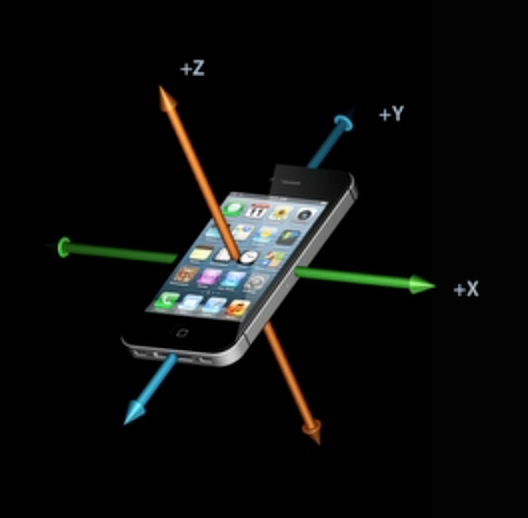
\includegraphics[width=0.4\textwidth]{figures/iphone_coordinatesystem}
    \caption{Depicts the iPhone's local coordinate system. Source:~\citep{apple:wwdc_2012_pham}}
    \label{fig:iphone_cs}
  \end{figure}
\end{center}

To start receiving the device's attitude via the \texttt{CMDeviceMotionManager} a reference frame needs to be specified. Figure~\ref{fig:iphone_cs}, shows the iPhones local coordinate system, which is important to know, to understand the differences between the four possible reference frames. The four \texttt{CMAttitudeReferenceFrame}s, illustrated in figure~\ref{fig:cm_referenceframes}, do have the vertical z-axis aligned with the gravity in common. According to \citet{apple:wwdc_2014_pham}, the specified reference frame, does also specify the type of sensor fusion. The following reference frames do exist \citep{apple:wwdc_2014_pham,apple:ios_doc_cm}:
\begin{itemize}
  \item \textbf{XArbitrary} (fig.~\ref{fig:cm_referenceframes_xArbitrary}): The x and y axis are unspecified. The initial pose fixes the x and y orientation. There is no heading correction; thus, it drifts over time.
  \item \textbf{XArbitraryCorrected} (fig.~\ref{fig:cm_referenceframes_xArbitraryCorrected}): The x and y axis are unspecified. The initial pose fixes the x and y orientation. Additionally, the magnetometer is used to correct heading and to improve yaw accuracy over time.
  \item \textbf{XMagneticNorth} (fig.~\ref{fig:cm_referenceframes_xMagneticNorth}): The x axis is absolutely tagged to magnetic north. It uses the compass for orientation.
  \item \textbf{xTrueNorth} (fig.~\ref{fig:cm_referenceframes_xTrueNorth}): The x axis is absolutely tagged to true north\footnote{The earth's magnetic field moves; thus, true and magnetic north are not the same. Maps are always oriented to true north.}. It uses the compass to determine true north.
\end{itemize}

\begin{figure}
      \subfloat[XArbitrary]{
        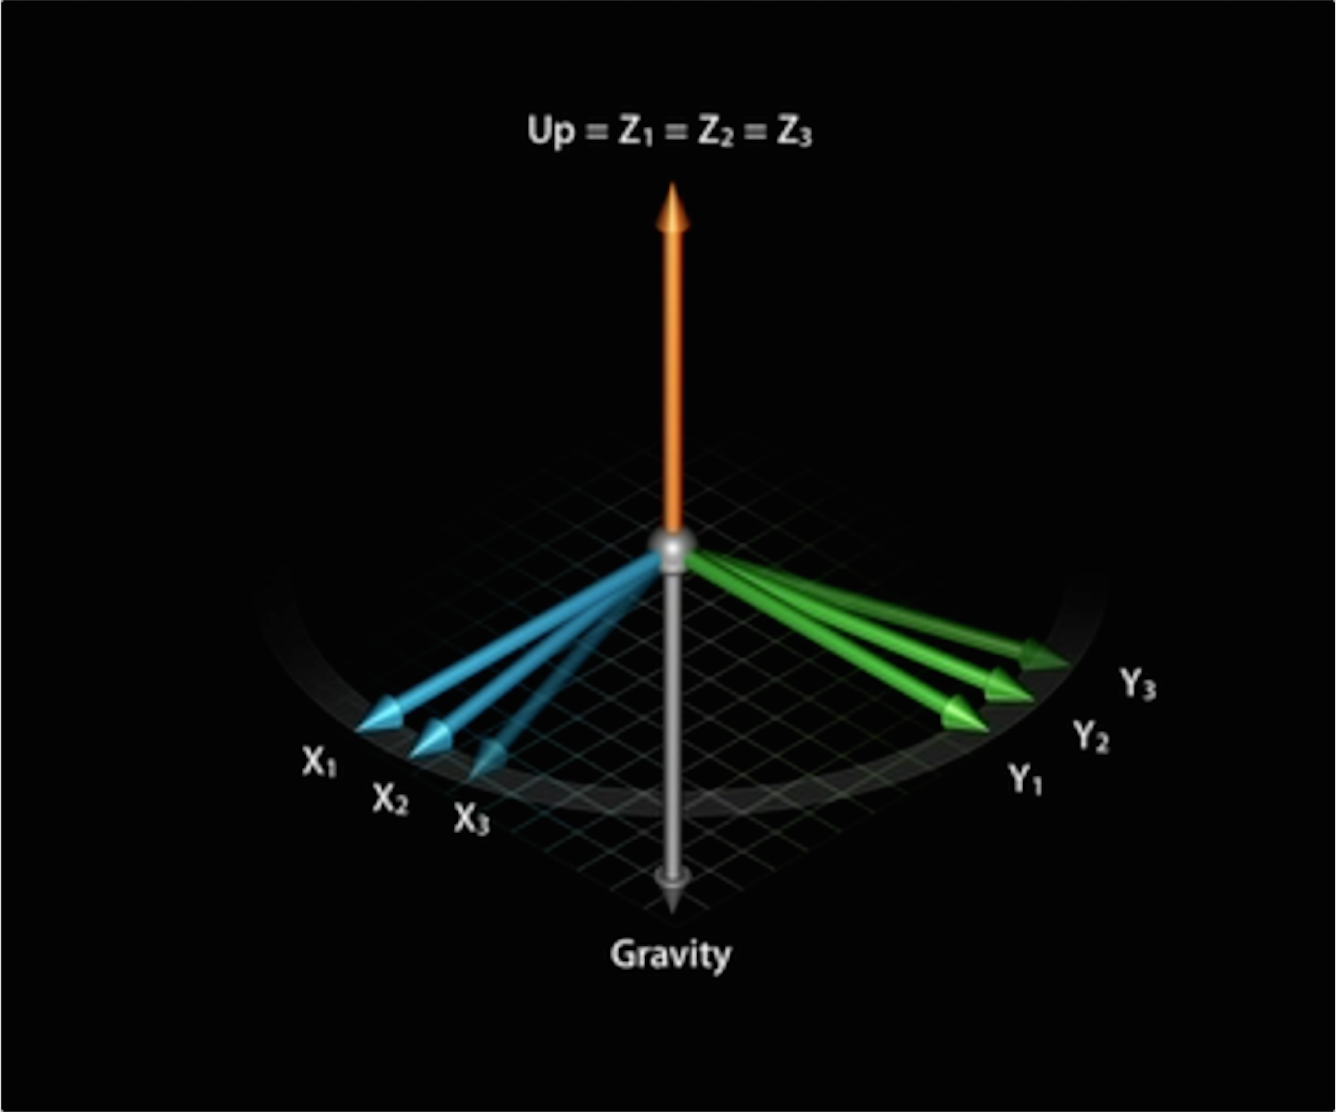
\includegraphics[width=0.4\textwidth]{figures/cm_xArbitrary}
        \label{fig:cm_referenceframes_xArbitrary}
      }
      \quad
      \subfloat[XArbitraryCorrected]{
        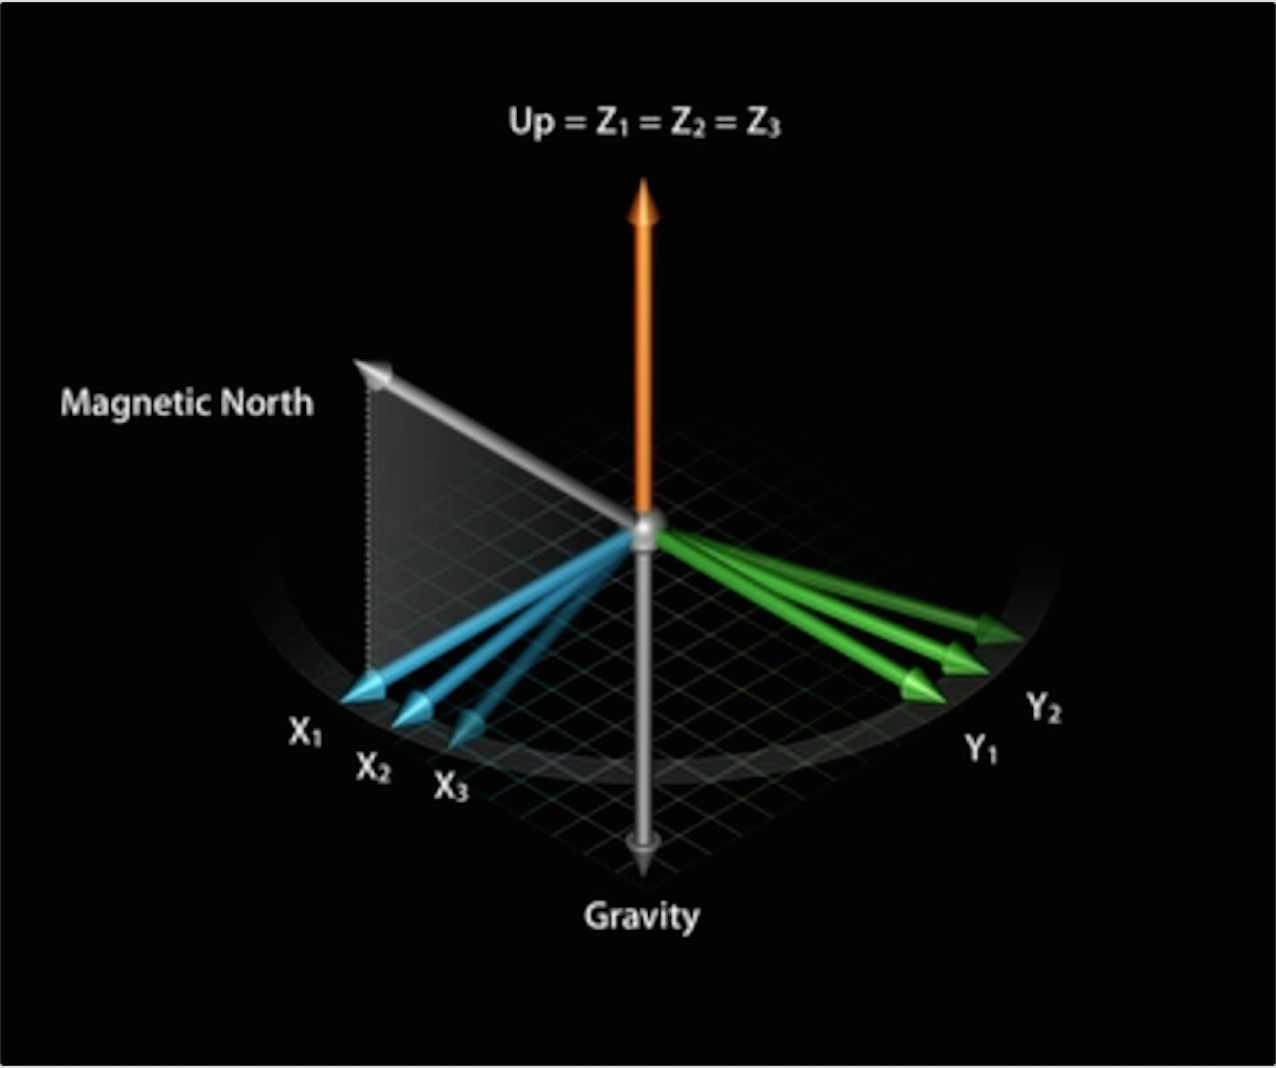
\includegraphics[width=0.4\textwidth]{figures/cm_xArbitraryCorrected}
        \label{fig:cm_referenceframes_xArbitraryCorrected}
      }
      \vspace{1cm}
      \subfloat[XMagneticNorth]{
        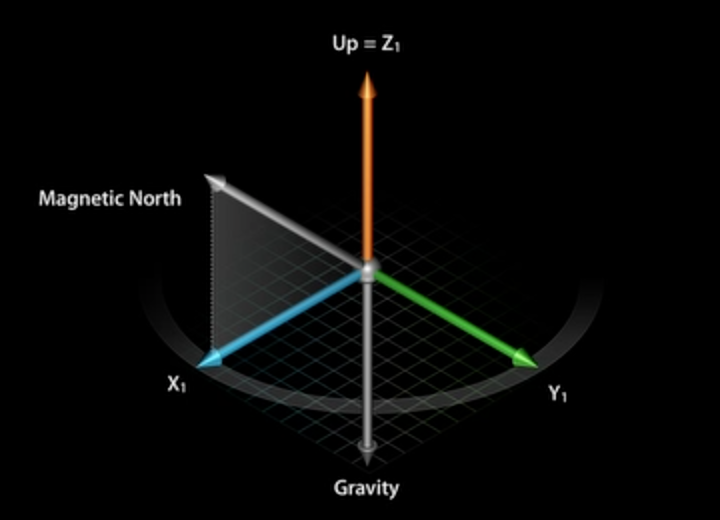
\includegraphics[width=0.4\textwidth]{figures/cm_xMagneticNorth}
        \label{fig:cm_referenceframes_xMagneticNorth}
      }
      \quad
      \subfloat[XTrueNorth]{
        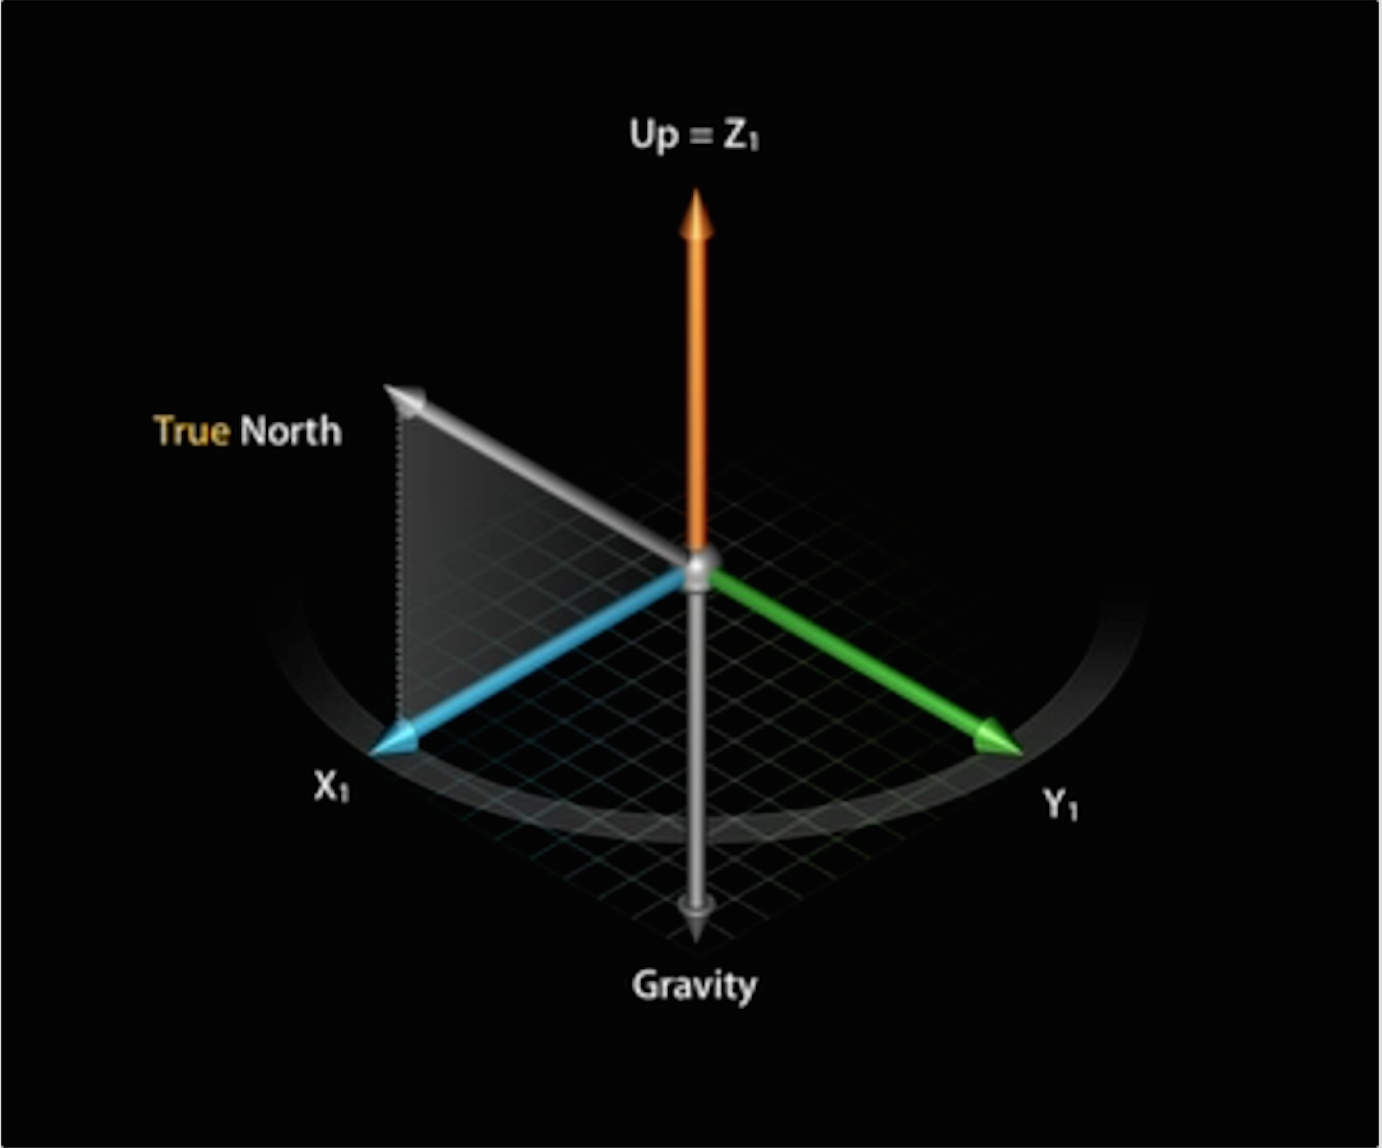
\includegraphics[width=0.4\textwidth]{figures/cm_xTrueNorth}
        \label{fig:cm_referenceframes_xTrueNorth}
      }
      \caption{Shows the different device attitude reference frames. Source: Andy Pham \cite{apple:wwdc_2012_pham}}
      \label{fig:cm_referenceframes}
\end{figure} % TODO Equal size


% sensor fusion accelerometer, gyro and depending on reference frame magnetometer
% gyro not for attitude, acc for tip and tilt but only under classy static state condition, and magnetometer good for heading other conditions interference
% pointing stability of the magnetometer and accelerometer and responsiveness of gyro
% sensor fusion removes uncertainties about ambiguities => gravity complete unconstraint motion, userAcceleration, rotationrate (bias compensated), attitude, and magneticfield (disturbance removed)
% user acceleration without gravity in G's 3 axis, without attitude it's assumtion is unclear how it looks if device is moved back and fourth
% rotation rate right hand rule
% all are by-products of attitude. Attitude pose in 3d space how it sits there.
% quaternions, rotationmatrix, euler angle
%reference frames => flavor of sensor fusion, xarbitrary -> z is align with gravitational axis uses initial value, xarbritrarycorrected uses magnetometer to corrected, better long term yaw accuracy
% true north, hiking should use true north because of maps.
\subsection{Compass}
The compass is part of the \ac{CL} framework. It provides the device's \emph{magnetic heading} and also its \emph{true north heading} in degrees. The heading depends on the specified device orientation, such as portrait, landscape left, or landscape right mode \citep{apple:ios_doc_cl}. According to \citet{apple:wwdc_2012_pham}, the compass uses sensor fusion and not only the magnetometer.

To access the device's heading, the \texttt{CLLocationManager} must be configured. It informs the application when the heading changes. The developer can specify a heading filter. Thus, a new heading is just reported, if the heading filter is exceeded \citep{apple:ios_doc_cl}.

As already mentioned before, the magnetometer measures the magnetic field, which is not just the earth's magnetic field. It is also being biased; for example, by iron bars and AC current. To reduce bias, the compass asks the user to calibrate it, by moving the device in a specific manner. \ac{CL} by itself can detect, if the compass needs calibration, and thus, automatically shows the user the calibration view \citep{apple:ios_doc_cl}.


\section{Evaluation}\label{sec:sensor_eval}
The purpose of this section is, to find out if the above referenced sensors and \acsp{API} are suitable for this project. Therefor, we evaluate the provided data, and also verify the above referenced statements, made by Apple's engineers.
% Verify apples statements
% evaluate the uncertainties


\subsection{MotionActivity}
As mentioned above, the \texttt{CMMotionActivity} component is to detect and classify a user's activity. To proof the statement concerning the recognition duration of the walking state, made by Apple's engineer \citet{apple:wwdc_2014_pham}, we did some test walks. The results of our experiment show, that the claim of a recognition time of 10--15~seconds, for the walking state, is very optimistic. Figure~\ref{fig:eval:motionActivity} shows the beginning of one of these test walks.

From the begin on, our test user started to walk with constant speed, with the phone in hand. The first line shows, that the component recognized, that the device is moving (not stationary), even before we started the application. In reality we first started the application, before we started to walk, but not stationary means that the user just somehow moves the device. After $\approx 10.7~\text{seconds}$, the component increases its confidence for the current state. Another $\approx 5~\text{seconds}$ later it set the confidence to high; thus, the component is very confident, that the user somehow moves the device. After $\approx 25~\text{seconds}$ of walking, the component finally detects, with medium confidence, that the user actually walks.

Compared to detecting the users walking state, it detects nearly in realtime, that the user stops walking after $\approx 32~\text{seconds}$. At this point in time, the user holds the device very steady, which is shown by the last three entries, where the component switches between stationary and not stationary, in a very short time period.

Our experiment shows, that the user needs to actually walk a very long distance, until the phone recognizes that the user is walking. It also shows, that the user has to hold the device very steady, until the device claims that the device is stationary. Consequently, \ac{CM}'s \texttt{CMMotionActivity} cannot really be used to determine a user's walking state, for short distances. Also the stationary state, cannot be used to claim that the user is not walking, due to the high sensibility.

\begin{figure}
\begin{tabular}{l*{7}{c}}
start date & confidence & unknown & stationary & walking & running & automotive & cycling \\
\hline
-2.0246 & 0 & false & false & false & false & false & false\\
10.7026 & 1 & false & false & false & false & false & false\\
15.7922 & 2 & false & false & false & false & false & false\\
25.9676 & 0 & false & false & \textbf{true} & false & false & false\\
32.3255 & 1 & false & \textbf{true} & false & false & false & false\\
32.6434 & 1 & false & false & false & false & false & false\\
33.2792 & 1 & false & \textbf{true} & false & false & false & false\\
\dots & \dots & \dots & \dots & \dots & \dots & \dots & \dots
\end{tabular}
\caption{Shows a part of the recorded MotionActivity during a test walk.
Remark: To simplify the table the start date is shown as relative timestamp instead of an absolute date.}
\label{fig:eval:motionActivity}
\end{figure}


\subsection{Pedometer}
To evaluate the accuracy of \ac{CM}'s \texttt{CMPedometer} component, we did some test walks for different distances, to compare the actual distance and step count, with the measured values. Due to the fact, that users usually carrying their smartphone in their pants pocket or holding it in their hand, we did the experiment for both positions. Figure~\ref{fig:eval:pedometerHand} shows the measured distances and the corresponding step counts, for different distances, with the phone in hand. The results of the same experiment with the phone in the pants pocket, are shown in figure~\ref{fig:eval:pedometerPocket}.

The experiments visualization shows the measurements dispersion. Sometimes, the \texttt{CMPedometer} overestimates or underestimates the distance, resp.\ the step count. It also shows, that the phone on average underestimates the values, if the user holds the device in hand. If the user walks with the phone in the pants pocket, the device also underestimates the measured distances; whereas, the measured step counts are more precise.

Figure~\ref{fig:eval:pedometerNDF} depicts the \texttt{CMPedometer}'s standard deviation $\sigma$, depending on the distance and phone's position. To model the uncertainty for any walked distance, depending on the phones position, we used linear regression based on our measurements. Initially, we expected a higher accuracy of the estimated distance, if the user carries the phone in the pants pocket, but the diagram proofs the opposite. Consequently, $\sigma$ is significantly smaller, if the user holds the phone in his hand.

%To be able to better compare the difference in the phone's position, we used the measured data to determine the pedometers uncertainties, depending on the walked distance. Figure~\ref{fig:eval:pedometerNDF} depicts the standard deviation $\sigma$, depending on the distance and phones position. To model the uncertainty for any walked distance, depending on the phones position, we used linear regression, based on our measurements. The difference in slope of the regression lines shows, that the phone in hand position provides a much better accuracy for increasing distances.

% CMPedometer (step count, distance)  dispersion plots
\begin{figure}
      \subfloat[Distance measurements]{
        \begin{tikzpicture}
          \begin{axis}[width=0.45\textwidth, height=0.4\textheight,
              xlabel={Reference distance (m)},
              ylabel={Distance (m)},
              legend entries={measurements, average},
              legend pos=south east,
            grid = major]
            \addplot [blue, only marks, mark=x] table[col sep=semicolon, x=distanceRef, y=distance] {csv/2014-10-28_htwg_keller_f/inHand.csv};
            \addplot [blue, only marks, mark=triangle*, mark size=3pt] table[col sep=semicolon, x=distanceRef, y=distance] {csv/2014-10-28_htwg_keller_f/inHand_avg.csv};
          \end{axis}
        \end{tikzpicture}
        \label{fig:eval:pedometerHand:dist}
      }
      \quad
      \subfloat[Step count measurements]{
        \begin{tikzpicture}
          \begin{axis}[width=0.45\textwidth, height=0.4\textheight,
              xlabel={Reference distance (m)},
              ylabel={Step count},
              legend entries={measurements, average, step count ref.},
              legend pos=south east,
            grid = major]
            \addplot [blue, only marks, mark=x] table[col sep=semicolon, x=distanceRef, y=steps] {csv/2014-10-28_htwg_keller_f/inHand.csv};
            \addplot [blue, only marks, mark=triangle*, mark size=3pt] table[col sep=semicolon, x=distanceRef, y=steps] {csv/2014-10-28_htwg_keller_f/inHand_avg.csv};
            \addplot [green, only marks, mark=*, mark size=3pt] table[col sep=semicolon, x=distanceRef, y=stepRef] {csv/2014-10-28_htwg_keller_f/inHand_avg.csv};
          \end{axis}
        \end{tikzpicture}
        \label{fig:eval:pedometerHand:steps}
      }
      \caption{Shows the measured distances and step counts for different distances. The measurements where taken indoor on a hard floor with the smartphone in hand.}
 \label{fig:eval:pedometerHand}
\end{figure}

\begin{figure}
  \vspace{1cm}
  \subfloat[Distance measurements]{
    \begin{tikzpicture}
      \begin{axis}[width=0.45\textwidth, height=0.4\textheight,
          xlabel={Reference distance (m)},
          ylabel={Distance (m)},
          legend entries={measurements, average},
          legend pos=south east,
        grid = major]
        \addplot [red, only marks, mark=x] table[col sep=semicolon, x=distanceRef, y=distance] {csv/2014-10-28_htwg_keller_f/inPocket.csv};
        \addplot [red, only marks, mark=triangle*, mark size=3pt] table[col sep=semicolon, x=distanceRef, y=distance] {csv/2014-10-28_htwg_keller_f/inPocket_avg.csv};
      \end{axis}
    \end{tikzpicture}
    \label{fig:eval:pedometerPocket:dist}
  }
  \quad
  \subfloat[Step count measurements]{
    \begin{tikzpicture}
      \begin{axis}[width=0.45\textwidth, height=0.4\textheight,
          xlabel={Reference distance (m)},
          ylabel={Step count},
          legend entries={measurements, average, step count ref.},
          legend pos=south east,
        grid = major]
        \addplot [red, only marks, mark=x] table[col sep=semicolon, x=distanceRef, y=steps] {csv/2014-10-28_htwg_keller_f/inPocket.csv};
        \addplot [red, only marks, mark=triangle*, mark size=3pt] table[col sep=semicolon, x=distanceRef, y=steps] {csv/2014-10-28_htwg_keller_f/inPocket_avg.csv};
        \addplot [green, only marks, mark=*, mark size=2pt] table[col sep=semicolon, x=distanceRef, y=stepRef] {csv/2014-10-28_htwg_keller_f/inPocket_avg.csv};
      \end{axis}
    \end{tikzpicture}
    \label{fig:eval:pedometerPocket:steps}
  }
  \caption{Shows the measured distances and step counts for different distances. The measurements where taken indoor on a hard floor with the smartphone in pants pocket.}
  \label{fig:eval:pedometerPocket}
\end{figure}

\begin{figure}
  \begin{tikzpicture}
    \begin{axis}[trim axis left, trim axis right, width=0.9\textwidth, height=0.4\textheight,
        xlabel={Distance / Mean $\mu$ (m)},
        ylabel={Standard deviation $\sigma$ (m)},
        legend entries={in hand, $f(\mu)=0.0971 \cdot \mu + 1.445$, in pocket, $f(\mu)=0.1971 \cdot \mu + 2.8703$},
        legend pos=north west,
      grid = major]
      \addplot [blue, mark=*] table[col sep=semicolon, x=mu_distanceRef, y=sigma_distanceRef] {csv/2014-10-28_htwg_keller_f/inHand_ndf_parameters.csv};
      %      \addplot [blue, dashed, domain=0:30, samples=2]{0.0680*x+2.1559};
      \addplot [blue, dashed, domain=0:30, samples=2]{0.0971*x+1.445};
      \addplot [red, mark=*] table[col sep=semicolon, x=mu_distanceRef, y=sigma_distanceRef] {csv/2014-10-28_htwg_keller_f/inPocket_ndf_parameters.csv};
      \addplot [red, dashed, domain=0:30, samples=2]{0.1971*x+2.8703};
    \end{axis}
  \end{tikzpicture}
  \caption {Shows the \texttt{CMPedometer} component's uncertainty, depending on the walked distance and the phone's position.}
  \label{fig:eval:pedometerNDF}
\end{figure}


Besides the pedometer's accuracy, we also evaluated the duration, until the component detects that the user is walking, and thus, delivers the first distance estimation. The \texttt{CMPedometer} component on average needs $5--10~\text{seconds}$ to deliver the first estimation, which is also consistent with statement made by \citet{apple:wwdc_2014_pham}. The first estimation typically contains a step count of $6--8~\text{steps}$. Once it detected that the user is walking, it continuously delivers estimation data, every $\approx 2.5 seconds$.

Another interesting value is the time it takes the pedometer, to recognize that the user continued walking, after a short break of $\approx 10--15~\text{seconds}$. Against our expectation, it takes approximately the same amount of time, and also the same amount of steps, as the component requires to recognize it the first time. This behavior is depicted in figure~\ref{fig:eval:pedometerExampleData}. Line 1 shows the amount of time and steps, it took the component, to recognize that the user is walking. After $50~\text{steps}$ the user took a short break of around $15 seconds$. The following lines show, that the component requires $6~\text{steps}$ to recognize, that the user continued walking. The third data block shows another break that the user made during the test walk.

\begin{figure}
\begin{tabular}{*{4}{l}}
startDate & endDate & distance & steps\\
\hline
0.0019 & 8.2329 & 4.8273 & 7\\
0.0019 & 10.7811 & 7.9850 & 11\\
0.0019 & 13.3238 & 11.4785 & 16\\
\dots & \dots & \dots & \dots\\
0.0019 & 31.1349 & 37.2110 & 50\\
0.0019 & 54.0149 & 37.2110 & 50\\
0.0019 & 56.5503 & 41.4032 & 56\\
\dots & \dots & \dots & \dots\\
0.0019 & 69.2608 & 57.2046 & 78\\
0.0019 & 84.5138 & 57.2046 & 78\\
0.0019 & 87.0569 & 64.8046 & 88
\end{tabular}
\caption{Shows the recorded pedometer example data.
Remark: To simplify the table, relative values for timestamp, startDate and endDate are being used, instead of the absolute timestamps. Additionally all values, except the steps, are being truncated.}
\label{fig:eval:pedometerExampleData}
\end{figure}


\subsection{Heading}
As mentioned earlier, our localization algorithm, introduced in chapter~\ref{chap:pf}, needs heading for the motion tracking, to determine in which direction the user is moving. To get the device's heading, either the \texttt{CMAttitude} provided by \ac{CM} or the \texttt{CLHeading}, provided by \ac{CL} can be used. In this paragraph we are first going to evaluate the \texttt{CMAttitude}'s data, and afterwards, the data provided by \texttt{CLHeading}.

%The device's attitude provided by the \texttt{CMDeviceMotion} component of Apple's CoreMotion framework can be used to calculate the device's heading.
\paragraph{CMAttitude} As mentioned before the \texttt{CMAttitude} data is being provided as Euler angles, Quaternions and as rotation matrix. To be able to compare attitude with compass heading, it is of advantage to transform the attitude into a heading in compass degrees. This means, if the device top is pointing towards magnetic north, the heading $\theta = 0^{\circ}$, east $\theta = 90^{\circ}$, south $\theta = 180^{\circ}$, and west $\theta = 270^{\circ}$. Equation~\ref{eq:rotationmatrix} shows the 3-dimensional rotation matrix provided by \texttt{CMAttitude}, as specified in the \ac{CM} framework's documentation \citep{apple:ios_doc_cm}. The calculation of $\theta$ in compass degrees, where $m_{1,2}$ and $m_{2,2}$ are describing the transformation of the phone's y-axis by the rotation around its z-axis, is shown in equation~\ref{eq:rotation2heading}.

\begin{equation} \label{eq:rotationmatrix}
  M_{3,3} = \begin{pmatrix}
      m_{1,1} & m_{1,2} & m_{1,3} \\
      m_{2,1} & m_{2,2} & m_{2,3} \\
      m_{3,1} & m_{3,2} & m_{3,3}
  \end{pmatrix}
\end{equation}

\begin{equation} \label{eq:rotation2heading}
  \theta = (\pi + {\rm atan2}\left(m_{2,2} , m_{1,2}\right)) \cdot \frac{180.0}{\pi}, \quad \text{for } m_{2,2}, m_{1,2} \neq 0
\end{equation}

As mentioned earlier, the \texttt{CMAttitude}'s values depend on the specified reference frame, which also affects the sensor fusion algorithm. To be able to easily compare the calculated heading $\theta$, directly with the compass heading, we decided to use the \texttt{xMagneticNorth} reference frame; thus, z is aligned to gravity, and x points towards magnetic north.

The most important requirement for heading is longterm accuracy. Therefor, we walked 10~times around a small table in same direction, and recorded the heading after each round. To record the heading we put the device after each round on the table, at the exact same position; thus, the heading should be roughly the same after each round. Figure~\ref{fig:evalAttitude:xMagneticNorth} illustrates the error of each measurement, compared to the initial measurement. First, we walked counter-clockwise around the table and observed an enormous drift of $\approx 30^{\circ}$ each round, which sums up to a drift of $\approx 300^{\circ}$ after 10 rounds. To double check this, we walked also clockwise around the table and observed the same amount of drift in the opposite direction. Apple's engineer, \citet{apple:wwdc_2014_pham}, explicitly mentioned that the magnetometer is being used to provide longterm yaw accuracy, if the \texttt{xArbitraryCorrected} reference frame is being specified. Thus, we repeated the same test for the \texttt{xArbitrary} and the \texttt{xArbitraryCorrected} reference frame, and compared it with the results before. Figure~\ref{fig:evalAttitude:referenceframes} shows the result. We found out, that there is nearly no difference in longterm accuracy, between the three tested reference frames.

% TODO Check reference (is it 2014 or 2012)

% heading calculation via rotation matrix
% statements regarding longterm accuracy
% reagiert nicht auf magnet

\begin{figure}[htbp]
    \begin{tikzpicture}
      \begin{axis}[width=0.5\textwidth, height=0.4\textheight,
          xlabel={round},
          ylabel={heading error (degree)},
          legend entries={counter-clockwise, clockwise},
          legend pos=north west,
        grid = major]
        \addplot [blue, mark=*] table[col sep=semicolon, x=round, y=error_attitude] {csv/deviceAttitudeAndCompass/xMagneticNorthAndCompass_left.csv};
        \addplot [blue, dashed, mark=*] table[col sep=semicolon, x=round, y=error_attitude] {csv/deviceAttitudeAndCompass/xMagneticNorthAndCompass_right.csv};
      \end{axis}
    \end{tikzpicture}
    \caption{Shows the heading's drift over time, calculated from \texttt{CMAttitude}, with reference frame \texttt{xMagneticNorth}.}
    \label{fig:evalAttitude:xMagneticNorth}
\end{figure}

\begin{figure}[htbp]
    \begin{tikzpicture}
      \begin{axis}[width=0.5\textwidth, height=0.4\textheight,
          xlabel={round},
          ylabel={heading error (degree)},
          legend entries={xMagneticNorth, xArbitrary, xArbitraryCorrected},
          legend pos=north west,
        grid = major]
        \addplot [blue, mark=*] table[col sep=semicolon, x=round, y=error_attitude] {csv/deviceAttitudeAndCompass/xMagneticNorthAndCompass_left.csv};
        \addplot [red, mark=*] table[col sep=semicolon, x=round, y=error_attitude] {csv/deviceAttitudeAndCompass/xArbitraryAndCompass.csv};
        \addplot [green, mark=*] table[col sep=semicolon, x=round, y=error_attitude] {csv/deviceAttitudeAndCompass/xArbitraryCorrectedAndCompass.csv};
      \end{axis}
    \end{tikzpicture}
    \caption{Shows the heading's drift over time, calculated from \texttt{CMAttitude}, with three different reference frames.}
    \label{fig:evalAttitude:referenceframes}
\end{figure}

\paragraph{CLHeading} During the experiment also the compass's \texttt{CLHeading} values, where recorded. Figure~\ref{fig:eval:compass} shows the heading's error over time. The values where measured together with the values of figure~\ref{fig:evalAttitude:xMagneticNorth} and \ref{fig:evalAttitude:referenceframes}. The chart shows no drift over time compared to the data measured from \texttt{CMAttitude}. But it also shows, that the compass can be biased by other magnetic fields. The outliers in the experiment with counter-clockwise direction let assume, that another magnetic field biased the before measured magnetic field.

That the compass reacts on other magnetic fields, than the earth's magnetic field, can easily by proofed by moving a small magnet around the phone. Compared to the compass, the \texttt{CMAttitude} does not react on other magnetic fields, like the one of a magnet.

According to the 40~measurements depicted in figure~\ref{fig:eval:compass}, the compass's standard deviation $\sigma$ amounts $3.1^{\circ}$. During the experiment, the \texttt{CLHeading} components heading filter, was set to $1.0^{\circ}$.
% compass ist genau genug

\begin{figure}[htbp]
  \begin{tikzpicture}
    \begin{axis}[width=0.6\textwidth, height=0.4\textheight,
      xlabel={round},
      ylabel={heading error (degree)},
      grid = major]
      \addplot [blue, mark=*] table[col sep=semicolon, x=round, y=error_compass] {csv/deviceAttitudeAndCompass/xMagneticNorthAndCompass_left.csv};
      \addplot [blue, dashed, mark=*] table[col sep=semicolon, x=round, y=error_compass] {csv/deviceAttitudeAndCompass/xMagneticNorthAndCompass_right.csv};
      \addplot [red, mark=*] table[col sep=semicolon, x=round, y=error_compass] {csv/deviceAttitudeAndCompass/xArbitraryAndCompass.csv};
      \addplot [green, mark=*] table[col sep=semicolon, x=round, y=error_compass] {csv/deviceAttitudeAndCompass/xArbitraryCorrectedAndCompass.csv};
    \end{axis}
  \end{tikzpicture}

  \caption{Shows the compass' magnetic heading error in degree. The measurements where taken by walking 10 times around a table. The initial measurement is being used as reference value. The heading filter was set to 1.0 degree.}
  \label{fig:eval:compass}
\end{figure}

\subsection{Summary}
As advertised, our solution, explained in chapter~\ref{chap:pf}, is based on \ac{MCL}. Therefor, we need motion tracking, which seems to be feasible by combining \ac{CM}'s distance estimation and \ac{CL} heading. If the \texttt{CLHeading} is heavily being influenced by other materials, like iron bars, it could probably being reasonable, to also integrate the discussed heading, based on \ac{CM}'s attitude. But, due to its huge drift problem, just the change in heading can be used.

\ac{CM}'s motion activity classification, seems to be useless, for our solution, due to its huge latency.